\cleardoublepage
\chapter{Learning MPC controllers with pQP neural networks}
\markboth{Learning MPC controllers with pQP neural networks}{Learning MPC controllers with pQP neural networks}

\section{Introduction}
\label{sec.chap4_intro}

Consider the standard MPC formulation for linear dynamical systems
\begin{subequations}
	\label{eq:linearmpc}
	\begin{align}
		%\mathds{P}1: \min_{X,U} \quad & q(x_H) + \sum_{k=1}^{H-1} l(x_k,u_k) \\
		\mathds{P}1: \min_{X,U} \quad & \sum_{k=0}^{N-1} \big( x_k^\top Q x_k + u_k^\top R u_k \big) + x_N^\top P x_N \label{eq.MPC_classical_cost}\\
		\text{subj. to} \quad 
		& x_{k+1} = A x_{k} + B u_{k}, \, \forall k = 0,\dots,N-1  \\
		& x_{k} \in \mathbb{X}, \, \forall k = 0,\dots,N-1 \\
		& u_{k} \in \mathbb{U}, \, \forall k = 0,\dots,N-1 \\
		& x_{H} \in \mathbb{X}_N \\
		& x_0 = x(0)
	\end{align}
\end{subequations}
where $x_k \in \mathbb{R}^{n_x}$, $u_k \in \mathbb{R}^{n_u}$, for all $k$; $X:=\{x_1,\dots,x_{N}\}$ and $U:=\{u_0,\dots,u_{N-1}\}$ are the collections of decision variables; $Q \succeq 0$, $R \succeq 0$ and $P \succ 0$ are cost matrices of adequate size; and the sets $\mathbb{X}$, $\mathbb{X}_N$ and $\mathbb{U}$ are polyhedra. Also, denote by 
\begin{equation}
	\pi: \mathcal{X} \rightarrow \mathbb{U}, \quad x(0) \mapsto \pi(x(0)) = u_0^\star
\end{equation} 
the mapping defined point-wise from the parameter $x(0)$ of $\mathds{P}1$ to the first control component of its optimizer\footnote{Since the objective is strictly convex and the constraints define a convex feasible set, if an optimizer exists for a given parameter $x(0)$, then this optimizer is unique.}. The domain $\mathcal{X} \subset \mathbb{R}^{n_x}$ is the collection of all $x(0)$ for which $\mathds{P}1$ is finite, i.e., the problem is feasible. It is well-known that, under reasonable standard on the terminal ingredients $P$ and $\mathbb{X}_N$, the map $\pi$ is a \ac{pwa} continuous function over a polyhedral partition of the polyhedron $\mathcal{X}$ \citep{bemporad2002explicit,borrelli2017predictive}. 

Automatic control involves real-time decision making and, in a number of different scenarios, it becomes infeasible or simply undesirable to solve an optimization problem such as \eqref{eq:linearmpc} on-line. Picture, for instance, a small embedded system that does not have enough computational resources to arrive at a solution within the time allocated to it. One method to circumvent solving $\mathds{P}1$ is to seek $\pi$, which can explicitly written in closed form with multi-parametric programming tools \citep{bemporad2002explicit}. This approach is known as explicit MPC and has become an establish control tool \citep{mariethoz2008explicit,naus2010design} for which free software exists \citep{herceg2013multi}. Unfortunately, $\pi$ can also be challenging both to compute and to store as the number of regions of its domain grows exponentially in the worst case with the number of inequality constraints in $\mathds{P}1$ \citep{alessio2009survey}, thus limiting its applicability. Simplifications strategies for explicit MPC exist, each coming with a different set (sometimes empty) of guarantees. In \cite{geyer2008optimal} and \cite{wen2009analytical}, for example, the authors build equivalent but more convenient representations of the control policy; in \cite{jones2008double} an incremental method is proposed to fit $\pi$ without requiring its explicit description; and in \cite{christophersen2007controller} and \cite{maddalena2019robust} safe elimination procedures are presented to drop certain regions without disrupting certain closed-loop properties.

%We assume a set of $N$ samples can be acquired from the original control law\footnote{The dataset can also be directly obtained from the implicit controller; depending on the size of the problem at hand, computing the explicit solution might be intractable.}
%\begin{subequations}
%	\begin{align}
%		& D = \{\text{x}_i,\text{u}_i\}_{i=1}^{N} \\[3pt]
%		& \text{u}_i = \pi(\text{x}_i), \; i=1,\dots,N
%	\end{align}
%\end{subequations}
%The process of acquiring the training dataset does not have to follow a particular distribution, nor do the samples have to be independent.

With the recent popularization of deep learning and the plethora of easy-to-use toolboxes available to users, \ac{nn} approximations of the map linking the current state $x(0)$ to the MPC optimal control action $u_0^\star$ have also become trendy (see e.g. \cite{karg2020efficient,kumar2021industrial}). Although the idea itself is not new \citep{parisini1995receding}, the latest investigations tend to make use of more modern analysis and synthesis tools such as better activation functions and training algorithms. The works \cite{fazlyab2020safety} and \cite{schwan2022stability} address the problem of verifying a NN approximation a posteriori, employing respectively semi-definite and mixed-integer linear programming techniques. On a different spirit, \cite{paulson2020approximate} tackles designing NNs that approximate predictive controllers and are safe by design. Arguably the main motivation behind this entire line of research is the expressive power of NNs, especially when deep architectures are employed \cite{karg2020efficient}, and the fact that they lie in the same class of \ac{pwa} functions as MPC controllers\footnote{As long as a \ac{pwa} activation function such as the rectified linear unit (ReLU) is used.}.

As opposed to the previously cited works where rather multi-purpose NN architectures were used, we will explore a structure that is tailored to the problem $\mathds{P}1$ and its solution $\pi$. Our proposal, which was published in \cite{maddalena2020neural} and \cite{maddalena2021embedded}, revolves around utilizing convex programs as layers within neural networks as proposed in \cite{amos2017optnet} and \cite{agrawal2019differentiable}. More specifically, the parameter to optimizer map of a convex program is employed as an internal layer, offering a particular inductive bias. A shallow architecture is proposed and shown to be able to represent the map $\pi$ of any predictive controller \eqref{eq:linearmpc} given a sufficiently large size. Finally, two examples are presented in the area of power electronics, allowing for a drastic speed-up in computation times with only a minor performance degradation.
	
\section{The proposed architecture}

An illustration of the \ac{pqp} neural network is shown in Figure~\ref{fig:nnArchitecture}. It is composed of two linear layers (L1 and L3), a single non-linear layer with adjustable parameters (L2), and a fixed output layer (L4). The central part of this structure is the \ac{pqp} layer L2, which is an implicit function described by the optimization model
%The key idea behind the proposed approximator is the use of a parametric quadratic program layer as part of the Neural Network, and optimizing over its parameters in order to fit the available dataset. This layer is implicitly described by the quadratic program
\begin{equation}
	\label{eq:pQP}
	y_2 = \text{arg}\,\min_{z \geq 0} \; ||Hz + y_1||^{2} + \epsilon ||z||^2
\end{equation}
that has $y_1$, the output of layer L1, as a parameter; the optimizer $y_2$ is then a function of $y_1$. Note how \eqref{eq:pQP} is always feasible and bounded from below, thus well posed for any $y_1$. The regularizing constant $\epsilon > 0$ is a fixed parameter that contributes with the numerical stability of the scheme. Additionally, if $\epsilon > 0$, then \eqref{eq:pQP} has always a unique minimizer and thus the map $y_1 \mapsto y_2$ is well defined.

Intuitively, one can think of the first layer L1 as a lifting, or projection, of the current state $x \in \mathbb{R}^{n_x}$ onto another space $\mathbb{R}^{n_z}$ whose dimension is a NN hyperparameter to be chosen by the user. L2 then is the key non-linear transformation that should capture most of the MPC policy complexity. Next, the affine map in L3 takes the $y_2$ value to the input space $\mathbb{R}^{n_u}$ and finally the control actions are guaranteed to satisfy the control constraints by projecting them onto $\mathbb{U}$, which is accomplished by L4 (see \eqref{def.pol_proj}). By adjusting $n_z$, the designer increases or reduces the representation power of the pQP NN although its size remains constant.
%which is \textit{always feasible} and \textit{bounded from below}. The size of this mathematical program, i.e. the dimension of $z$, can be tuned to attain approximations with different complexity. Moreover, as notation suggests, the parameter $y_1$ depends on a previous affine layer that maps the system states into the $z$ space, $y_1 := Fx + f$. Let $y_2 := z^{\star}$, then another affine layer maps the optimal solution to the input space $y_3 := Gy_2 + g$, and a projection onto the feasible input set produces the final control action $\hat{u} := \text{Proj}_{\, \mathbb{U}}(y_2)$. This last step is necessary to guarantee feasibility of the control moves (see e.g. \cite{chen2018approximating}). An illustration of the proposed architecture is presented in Fig.~\ref{fig:nnArchitecture}, where the projection layer was particularized to a familiar element-wise saturation operation $\text{sat}(\cdot)$, valid for box input constraints.

\begin{figure}[t!]
	\begin{center}
		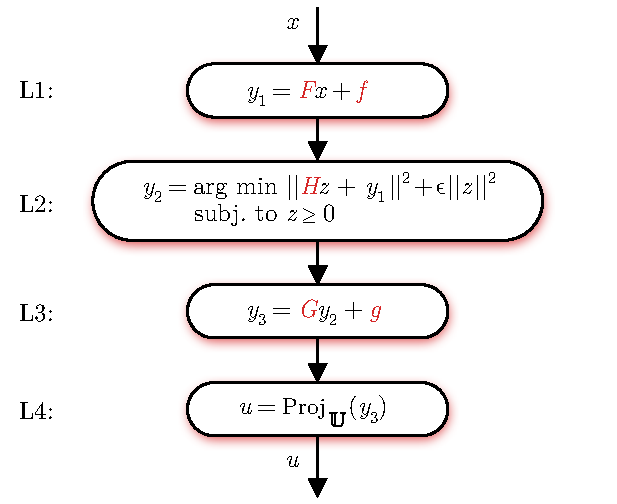
\includegraphics[scale=0.8]{../images/chap4_nn_arch.pdf}  
		\caption{A pQP neural network architecture tailored to MPC. The variables in red are weights to be adjusted during training.}
		\label{fig:nnArchitecture}
	\end{center}
\end{figure}

%Let the chosen number of decision variables in the pQP be $z \in \mathbb{R}^{n_z}$. We choose $L \in \mathbb{R}^{n_z \times n_z}$ to be square, and therefore $F \in \mathbb{R}^{n_z \times n}$, $f \in \mathbb{R}^{n_z}$. Moreover, $G \in \mathbb{R}^{m \times n_z}$ and $g \in \mathbb{R}^{m}$. If $n_z \ge n$, the first layer lifts the input data into a higher dimensional space before it is passed through the optimization layer. A last affine function then projects it onto the control space. These facts will be later employed to analyze the representative power of the network.
Let $\hat\pi : x \mapsto u$ be the pQP NN map defined by the composition of the layers in Figure~\ref{fig:nnArchitecture}, and whose parameters to be trained are $F \in \mathbb{R}^{n_z \times n_x}$, $f \in \mathbb{R}^{n_z}$, $H \in \mathbb{R}^{n_z \times n_z}$, $G \in \mathbb{R}^{n_u \times n_z}$ and $g \in \mathbb{R}^{n_u}$. The final goal is to tune these to fit a dataset of the form 
\begin{equation}
	\{(x(0)_i, u_{0,i}^\star)\}_{i=1}^d
\end{equation}
composed of initial conditions $x(0)$ and the first optimal control action $u_0^\star$ coming from \eqref{eq:linearmpc}. Typically, this is done by defining a suitable loss function and minimizing the mismatch between $\hat\pi(x(0))$ and $u^\star_0$, i.e., the control action produced by the pQP NN and the target optimal value. The parameters are then tuned by means of a gradient-based  backpropagation procedure. 

\begin{remark}
	As shown in \cite[Theorem~1]{amos2017optnet}, OptNet layers are differentiable everywhere, but not in a set of measure zero of parameters, where subgradients exist. Since \eqref{eq:pQP} is a particular instance of the OptNet layer, it inherits its properties. Moreover, we assume the set of feasible control actions $\mathbb{U}$ to be a polyhedron. The projection operator in L4 is therefore a quadratic program with $y_3$ as its only parameter and, thus, also an OptNet layer.
\end{remark}

%This process can be carried out via a stochastic gradient descent algorithm applied to an appropriate loss function. Differentiability of all layers is trivial with the exception of the pQP one \citep{gould2016differentiating,amos2017optnet}. Regarding the latter, note that the objective in \eqref{eq:pQP} can be rewritten as
%\begin{equation}
%	\label{eq:idk}
%	V(z) := z'(\epsilon I + L'L)z + (2L'y_1(x))' \, z + y_1(x)'y_1(x)
%\end{equation}
%whose Lagrangian is simply
%\begin{equation}
%	\mathcal{L}(z,\lambda) = V(z) - \lambda'z
%\end{equation}
%The Karush-Kuhn-Tucker (KKT) conditions for primal and dual feasibility, complementary slackness, and stationarity then read 
%\begin{subequations}
%	\label{eq:kkt}
%	\begin{align}
%		& z^\star \geq 0 \\
%		& \lambda^\star \geq 0 \\
%		& \lambda_i^\star z_i^\star = 0, \ \forall i = 1,\dots,n_z \\
%		& 2(\epsilon I + L'L)z^\star + (2L'y_1(x)) - \lambda^\star = 0
%	\end{align}
%\end{subequations}
%where $\lambda_i$ and $z_i$ denote the components of the Lagrange multipliers and decision variables vectors. The following proposition presents the differentiability properties of the pQP layer, and holds since \eqref{eq:pQP} is a particular instance of the \texttt{OptNet} layer \citep{amos2017optnet} with strictly convex objective function.
%
%\begin{proposition}
%	Let $\theta := (L,y_1)$. The parametric solution $z^\star(\theta)$ of \eqref{eq:pQP} is subdifferentiable everywhere in its domain, i.e., $\partial z^\star(\theta) \neq \{ \, \}$, and $\partial z^\star(\theta)$ has a unique element (the jacobian) everywhere but in a set of measure zero.
%\end{proposition}
%As shown in \cite{amos2017optnet}, the relevant gradients with respect to the parameters to be trained can be obtained from the KKT set of equations \eqref{eq:kkt}. Hence, backward passes are possible and backpropagation can be performed to optimize all of the NN parameters.

\section{Properties of the approximator}
\label{sec.properties_approx}
%Depending on the number of parameters $n_z$, and thus on the size of the NN, the proposed architecture can not only approximate arbitrarely well, but generate exactly any continuous piecewise affine function. The formal statement is presented next.
%The authors of \cite{hempel2013every} showed that any continuous PWA function can be obtained as the solution of a particular parametric linear program (pLP) transformed by a linear map. Even though this view could be adopted herein, we instead prove a different result that is enough in the context of linear eMPC.
Regard the size $n_z$ in L2 as a hyperparameter. It is then clear that as $n_z$ increases, the expressive power of the pQP NN also increases. Moreover, as $\hat\pi$ is defined by a composition of piece-wise affine functions, it is itself piece-wise affine. Next we prove that $\hat\pi$ can not only approximate well any linear MPC controller, but also recover an exact representation if an appropriate size $n_z$ is chosen.

\begin{theorem}
	\label{thm:pQPrepr}
	\textbf{(The pQP NN can learn any linear MPC controller):} Let $\hat{\pi}: \mathbb{R}^{n_x} \rightarrow \mathbb{R}^{n_u}$ be the map defined by the composition of all four layers, i.e., $\hat{\pi}(x) := L4 \circ L3 \circ L2 \circ L1(x)$. Set $\epsilon = 0$, then $\exists F$, $f$, $H$, $G$ and $g$ with appropriate dimensions such that $\forall x \in \mathcal{X}, \ \hat{\pi}(x) = \pi(x)$.
\end{theorem}

\textit{Proof}: In essence, the proof consists in showing that L2 has exactly the same structure as the dual of the MPC formulation \eqref{eq:linearmpc}, and in showing that L3 can recover the primal solution from the dual.

Start by condensing the MPC problem $\mathds{P}1$, i.e., using the equality constraints to eliminate all state decision variables except for the initial state $x(0)$. This leads to the following parametric problem
\begin{subequations}
	\begin{align}
		%\mathds{P}1: \min_{X,U} \quad & q(x_H) + \sum_{k=1}^{H-1} l(x_k,u_k) \\
		\mathds{P}2: \min_{U} \quad & U^\top \, \Lambda \, U + x(0)^\top \, \Gamma \, U\\
		\text{subj. to} \quad & \Phi \, U \leq  \Omega \, x(0) + \omega \label{eq:constr}
	\end{align}
\end{subequations}
The step by step condensing procedure can be found in \cite{wright2019efficient}, which also shows that $\Lambda \succ 0$. The problems $\mathds{P}2$ and $\mathds{P}1$ are then equivalent in the sense that the solutions $U^\star$ of $\mathds{P}2$ and $(X^\star,U^\star)$ of $\mathds{P}1$ share the same $U^\star$ component. Next, derive the dual problem of $\mathds{P}2$, which is
%\begin{equation} 
%		\label{eq:dualMPC} 
%		\mathds{D}2: \min_{\lambda \geq 0} \ \frac{1}{4} \, \big[ \lambda^\top\Phi \, \Lambda^{-1}\Phi^\top\lambda + \, (4 x(0)^\top\Omega^\top+2 x(0)^\top\Gamma \Lambda^{-1} \, \Phi^\top + 4 \omega')\lambda + \, x(0)^\top\Gamma \Lambda^{-1} \Gamma^\top x(0) \big]
%\end{equation}
\begin{equation}
	\begin{split} 
		\label{eq:dualMPC} 
		\mathds{D}2: \min_{\lambda \geq 0} \ \frac{1}{4} \, \big[ \lambda^\top\Phi \, \Lambda^{-1}\Phi^\top\lambda + \, (4 x(0)^\top\Omega^\top+2 x(0)^\top\Gamma \Lambda^{-1} \, \Phi^\top + 4 \omega^\top)\lambda \dots \\
		+ \, x(0)^\top\Gamma \Lambda^{-1} \Gamma^\top x(0) \big]
	\end{split}
\end{equation}
And use the KKT stationarity condition of $\mathds{P}2$ to arrive at an expression that relates linearly the optimal primal and dual solutions
%It is possible to recover the primal optimal solution $U^\star$ from the dual optimal solution $\lambda^\star$ through the stationarity optimality condition of $\mathds{P}2$
\begin{equation}
	\label{eq:stationarity}
	U^\star = -0.5 \, \Lambda^{-1}\Phi^\top \lambda^{\star} -0.5 \, \Lambda^{-1} \Gamma^\top x(0)
\end{equation}
%Next, it would be possible to enforce the first two layers to match the dual problem $\mathds{D}2$, and the third to implement \eqref{eq:stationarity} and recover the primal solution. Nevertheless, this would require the third layer to have a so called skip connection directly from the NN input, i.e., access to $x(0)$. We instead define slightly different linear and pQP layers that not only learn $\mathds{D}2$, but also let $x(0)$ pass through them and arrive at the second linear layer.
%The above equation is learned by the second linear layer in Figure~\ref{fig:nnArchitecture}. Nevertheless, from \eqref{eq:stationarity} we see that it requires the value of $x(0)$, which is the NN input. It is shown next that with a pQP layer of appropriate size and parameters, it is possible not only to learn \eqref{eq:dualMPC}, but also let the value of $x(0)$ `pass through' the NN and arrive to the second linear layer as needed to retrieve the primal optimal solution.
Next, rewrite L2 in the standard QP form
\begin{equation}
	\label{eq:L2_qpform}
	\min_{z \geq 0} \ z^\top(H^\top H + \epsilon I )z + (2H^\top y_1)^\top \, z + y_1^\top y_1
\end{equation}
and match\footnote{The last terms of the two QPs are disregarded since their are independent of the optimization variables and thus have no effect on their respective optimizers.} the two quadratic programs \eqref{eq:dualMPC} and \eqref{eq:L2_qpform} through  %Let the auxiliary variable $\tilde{L}$ and function $\tilde{y}_1(x) := \tilde{F}x + \tilde{f}$ be the solution to (compare \eqref{eq:idk} and \eqref{eq:dualMPC})
\begin{subequations}
	\label{eq:Landg1}
	\begin{align}
		\tilde{H}^\top \tilde{H} + \epsilon I & = 0.25 \, \Phi \Lambda^{-1} \Phi^\top \\
		2 \tilde{H}^\top \tilde{y}_1 & = \Omega \, x(0) + 0.5 \, \Phi \Lambda^{-1}x(0) + \omega %\\
		%y_1(x)'y_1(x) & = 0.25 \, \overline{r}'\overline{R}^{-1}\overline{r}
	\end{align}
\end{subequations}
which leads to $\epsilon = 0$, $\tilde{H} = 0.5 \, (\Phi \Lambda^{1/2})^\top$, and $\tilde{y}_1 = (\Phi \Lambda^{1/2})^{-1} (\Omega \, x(0) + 0.5 \, \Phi \Lambda^{-1} x(0) + \omega).$ This value of $\tilde y_1$ also defines the weights $F$ and $f$ of the L1 layer simply as $\tilde{F} = (\Phi \Lambda^{1/2})^{-1}(\Omega+0.5 \, \Phi \Lambda^{-1})$ and $\tilde{f} = (\Phi \Lambda^{1/2})^{-1}\omega$. 

Tilde superscripts were used for $H$, $y_1$, $F$ and $f$ in the last paragraph because those are not the final values of those parameters. Indeed, they need to be augmented to resolve the following issue. For the layer L3 to implement \eqref{eq:stationarity}, it would need access to $x(0)$, whereas it only receives $y_2$ from the previous layer. The solution lies in augmenting L1 and L2 to match the MPC dual as previously done and, in addition, also let the NN input $x(0)$ pass through them and arrive at L3. More concretely, the steps below have to be followed.

Set the first layer weights to $F = [-I \ I \ \tilde{F}]^\top$ and $f = [0 \ 0 \ \tilde{f}]^\top$ so that $y_1 = [-x \ x \ \tilde{F}x + \tilde{f}]^\top$. Set the L2 weights to $\epsilon = 0$ and $H = [I \ 0 \ 0; \,0 \ I \ 0; \, 0 \ 0 \ \tilde{H}]$. Partitioning the decision vector into three components $z = [x^p \ x^n \ \tilde{z}]^\top$ leads to
\begin{equation}
	% \small
	\label{eq:pQPtilde}
	\min_{\tilde{z},x^p,x^n \geq 0} \, ||x^p - x(0)||^{2} + ||x^n + x(0)||^{2} + ||\tilde{H}\tilde{z} + \tilde{y}_1||^{2} 
\end{equation}
which is a separable objective in $\tilde{z}$, $\tilde{x}^p$ and $\tilde{x}^n$. Thanks to the choice of $\tilde{L}$ and $\tilde{y}_1$ we have that $\tilde{z}^\star$ in \eqref{eq:pQPtilde} matches $\lambda^\star$ in \eqref{eq:dualMPC}. Regarding $x^{p\star}$, the $n$th optimizer components will satisfy $\forall i = 1,\dots,n$, $x^{p\star}_i = x_i(0)$ if $x_i(0) \geq 0$, else $x^{p\star}_i = 0$. Similarly, $x^{n\star}_i = -x_i(0)$ if $x_i(0) \leq 0$, else $x^{n\star}_i = 0$. Therefore, $x^{p\star} - x^{n\star} = x(0)$, and the output of the pQP layer \eqref{eq:pQPtilde} will contain the dual optimizer $\lambda^\star$ and the NN input value $x(0)$ encoded in it.

Next set the weights of L3 to match \eqref{eq:stationarity}, but only extracting the first optimal control action rather than the whole vector. This is accomplished by $G = \nabla\, [-0.5 \Lambda^{-1}\Gamma^\top \ \ 0.5\Lambda^{-1}\Gamma^\top \ - 0.5 \Lambda^{-1}\Phi^\top ]$ and $g = 0$. Therefore, $y_3 = G \, [x^{p \star} \ x^{n\star} \ \tilde{z}^\star ]^\top = G \, [x^{p \star} \ x^{n\star} \ \lambda^\star]^\top = \nabla\, U^\star = u_0^\star$, where $\nabla$ is a matrix containing zeros everywhere and a $n_u \times n_u$ identity matrix in its lower right corner.

Finally, note that L4 will evaluate to $u_0^\star$ since $y_3 = u_0^\star$ necessarily belongs to $\mathbb{U}$. The proof is concluded after observing that the value of $x(0)$ in the above calculations can be taken to be any point $x$ in $\mathcal{X}$. $\square$

\begin{remark}
	Given a large enough size $n_z$, $\hat\pi(x)$ can match $\pi(x)$ under appropriate parameters. In practice however, one is rather interesting in experimenting with small sizes $n_z$ to reduce the complexity of the final map.
\end{remark}

\begin{remark}
	As opposed to $\pi(x)$, $\hat\pi(x)$ is defined for any $x \in \mathbb{R}^{n_x}$.
\end{remark}

The deployment of the pQP NN does not have to involve solving L2 on-line. Indeed, its explicit solution could be found off-line, in which case the real-time evaluation of $\hat\pi(x)$ would boil down to computing affine and piece-wise affine expressions. By adjusting $n_z$, the designer can therefore tune $\hat\pi(x)$ to its needs. The whole process can be than seen as the fitting of a PWA function, the pQP NN, to another PWA function, the MPC explicit solution.

Approximating the MPC controller \eqref{eq:linearmpc} with our network architecture does not come with \textit{a priori} guarantees on closed-loop stability or convergence to an equilibrium point. Nevertheless, once the pQP NN is trained, tools from mixed-integer programming can be exploited to compute the worst-case mismatch between $\pi(x)$ and $\hat\pi(x)$ as well as basins of attraction for the closed-loop system \citep{schwan2022stability}. Alternatively, a robust MPC controller could be designed taking into account a certain level of input disturbace, which will be incurred later by the approximation scheme. This is the idea proposed in \cite{hertneck2018learning}, where statistical guarantees are derived based on samples, and without needing access to the worst-case approximation error. Finally, safety filters could be employed not to certify the pQP NN, but to modify minimally its control actions to ensure system theoretical properties \citep{wabersich2018linear}.

\section{Numerical validation}

In this section we make use of the previously proposed architecture to approximate the MPC controller of a 4-state, 3-input model of a multi-cell DC-DC power converter. The size $n_z$ is then varied and its effect on the quality and size of the approximate solution is studied.

\subsection{The dynamics and the target predictive controller}
\label{sec:analysis}

Parallelism is a key concept to increase the efficiency and power levels of electronic converters. Still, this design choice has to be followed by proper current and voltage balancing techniques to ensure that no single stage is subjected to a exceedingly high electrical stress when compared to the others. 

A schematic representation of a multi-cell step-down converter is shown in Figure~\ref{fig.multi-cell}, and its parameters can be found in Table~\ref{tab_multi_cell}. The topology features three arms that are connected to a coupled inductor, and an L-C output filter. All self inductances are assumed equal $L_1 = L_2 = L_3 = L_{s}$, and all mutual inductances have value $L_m$. The switches of each arm operate in a complementary fashion at a fixed frequency $f = \,$15 kHz, and with variable but constrained duty cycle $0 \leq d_i \leq 0.9, \, i=1,2,3$. Let the average voltage applied by the arms over one switching period be denoted by $v_i := d_i V_{in}, i=1,2,3$. In order to ease the analysis, we apply the Lunze transform $\Psi$ to all variables, decomposing the phase voltages and currents into differential and common mode components
\begin{align}
	% \begin{bmatrix}
	%     i_{dm1} \\ i_{dm2} \\ i_{cm}  
	% \end{bmatrix} 
	% := \Gamma 
	% \begin{bmatrix}
	%     i_{1} \\ i_{2} \\ i_{3}
	% \end{bmatrix}
	\begin{bmatrix}i_{dm1} & i_{dm2} & i_{cm}\end{bmatrix}^\top &:= \Psi \, \begin{bmatrix}i_{1} & i_{2} & i_{3}\end{bmatrix}^\top \\
	% \begin{bmatrix}
	%     v_{dm1} \\ v_{dm2} \\ v_{cm}  
	% \end{bmatrix} 
	% := \Gamma 
	% \begin{bmatrix}
	%     v_{1} \\ v_{2} \\ v_{3}
	% \end{bmatrix}
	\begin{bmatrix}v_{dm1} & v_{dm2} & v_{cm}\end{bmatrix}^\top &:= \Psi \, \begin{bmatrix}v_{1} & v_{2} & v_{3}\end{bmatrix}^\top
\end{align}
where $\Psi = (1/3) \, [2 \, -1 \, -1; \, -1 \ \, 2 \, -1; \, 1 \ \, 1 \ \, 1]$.

The control input is defined as $u := [v_{dm1} \; v_{dm2} \; v_{cm}]^\top $ and the continuous-time state vector, by appending the output voltage to the transformed currents $x := [i_{dm1} \; i_{dm2} \; i_{cm} \; v_{out}]^\top $. By using Kircchoff's circuit laws, a linear model of the form $\dot{x} = A_{ct} x + B_{ct} u$ can be derived with

\begin{equation}
	\small
	A_{ct} = 
	\begin{bmatrix}
		\frac{-R}{L_s - L_m} & 0 & 0 & 0 \\
		0 & \frac{-R}{L_s - L_m} & 0 & 0 \\
		0 & 0 & \frac{-R}{L_s + 2L_m + 3L_f} & \frac{-1}{L_s + 2L_m + 3L_f} \\ 
		0 & 0 & \frac{3}{C_o} & \frac{-1}{R_o C_o}
	\end{bmatrix}
\end{equation}
\begin{equation}
	\small
	B_{ct} = 
	\begin{bmatrix}
		\frac{1}{L_s-L_m} & 0 & 0\\
		0 & \frac{1}{L_s-L_m} & 0 \\
		0 & 0 & \frac{1}{L_s + 2L_m + 3L_f} \\ 
		0 & 0 & 0
	\end{bmatrix}
\end{equation}
Finally, discretization at frequency $f$ is carried out using the zero-order hold method, yielding $x_{k+1} = A x_{k} + B u_{k}$.

\begin{figure}[!t]
	\centering
	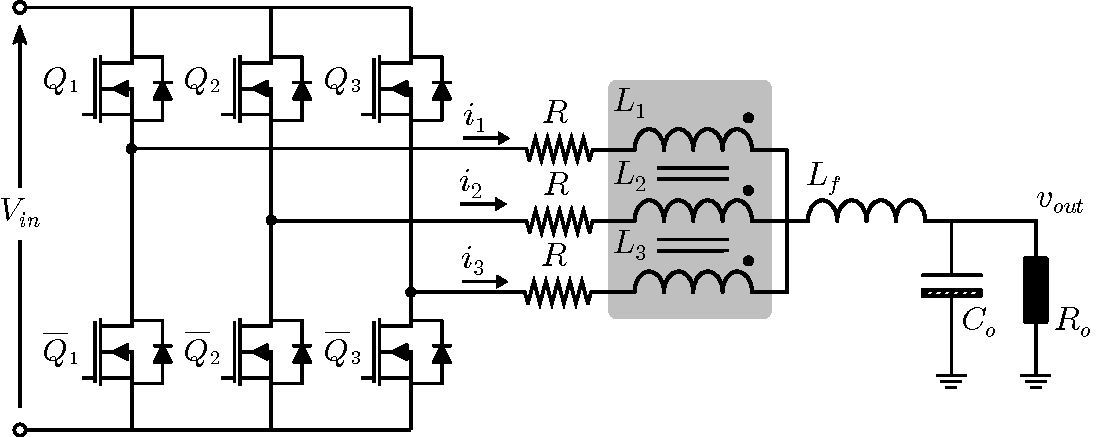
\includegraphics[width=0.7\linewidth]{../images/chap4_simres_multicelldcdc}
	\caption{A diagram of the multi-cell step-down DC-DC converter.}
	\label{fig.multi-cell}
\end{figure}

The control goal is to regulate the output voltage $v_{out}$ to 300$\,$V while maintaining the phase currents balanced at all times, which translates to driving the differential currents to zero. More specifically we have the following  fixed reference $x_{eq} = [0 \; 0 \; 16 \; 300]^\top $ with $u_{eq} = B^{\dagger}(I-A)x_{eq}$, where $B^\dagger$ denotes the pseudo-inverse of $B$. Moreover, the controller approximation procedure must not incur a steady-state error larger than 200$\,$mA for $i_{dm1}$ and $i_{dm2}$, and 5\% for the common mode component $i_{cm}$ and output voltage $v_{out}$. The chosen MPC cost function was\footnote{$||a-b||_C^2 := (a-b)^\top C (a-b)$.}
\begin{equation}
	\label{eq.MPC_cost_tracking}
	J = \sum_{k=0}^{N-1} (||x_{k}-x_{eq}||_Q^2 + ||u_{k}-u_{eq}||_R^2) \, + \, ||x_{N}-x_{eq}||_P^2
\end{equation}
where $Q = \text{diag}(10, \, 10, \, 0.1, \, 0.1)$, $R = 0.1 \, I$, $P$ is the solution to the associated the discrete-time algebraic Riccati equation, and $N=10$. For all time instants, box state constraints were imposed $\begin{bmatrix}-5 & -5 & -10 & -20\end{bmatrix}^\top  \leq x_{k} \leq \begin{bmatrix}5 & 5 & 30 & 400\end{bmatrix}^\top$ and polyhedron constraints on the controls $H_u \, u_k \leq h_u$ that simply mapped the duty cycle saturation to the Lunze domain. Due to the polytopic input constraints, the system cannot be decomposed into three decoupled parts as the structure of matrices $A_{ct}$ and $B_{ct}$ suggest. Furthermore, the standard terminal set constraint was imposed on $x_N$, defined as the invariant set associated to the unconstrained infinite-time problem formulation.

\begin{table}[!t]
	\begin{center}
		\caption{The parameters of the multi-cell step-down DC-DC converter.} 
		\label{tab_multi_cell}
		\begin{tabular}{c c c c c c c c}
			\cmidrule[.15em](l{\tabcolsep}r{\tabcolsep}){1-8}
			$V_{in}$ & $L_{s}$ & $L_{m}$ & $R$ & $L_f$ & $C_o$ & $R_o$ & \\
			\cmidrule[.05em](l{\tabcolsep}r{\tabcolsep}){1-8}
			350$\,$V & 4$\,$mH & -2$\,$mH & 10$\,$m$\Omega$ & 270$\, \mu$H & 20$\, \mu$F & 6.25$\, \Omega$ \\ 
			\cmidrule[.15em](l{\tabcolsep}r{\tabcolsep}){1-8}
		\end{tabular}
	\end{center}
\end{table}

With the aid of the Multi-Parametric Toolbox (MPT) for MATLAB \citep{herceg2013multi}, the explicit MPC solution $\pi(x)$ was computed and consisted of 2'337 regions. By counting the number of parameters of each halfspace and control gain, the memory requirement of this PWA function was found to be 518$\,$kB, considering a 4-byte representation for both integers and floating point numbers.


\subsection{Learning the optimal controller}

A total of 5'000 samples were acquired from the explicit MPC policy using a uniform distribution across the state-space. The dataset outputs $u_{0i}^\star$ were then normalized since their first two components had considerably low amplitudes compared to the third due to the structure of the Lunze transform $\Psi$. Instead of implementing a general projection operator in L4, the layer was simplified to $u = \Psi \, \text{sat}(y_3)$ with saturation limits $0$ and $0.9 \, V_{in}$, which clearly guarantees control feasibility without the need of a second quadratic program. Several pQP NNs were then trained with $n_z=1,\dots,7$.  The MPC approximators were trained using \texttt{PyTorch} and the \texttt{OptNet} frameworks, and mean squared error loss function. Mini-batch stochastic gradient descent with Adam \citep{kingma2014adam} was the optimization algorithm of choice to minimize the loss with batch size of $50$ and $150$ epochs. Training a single pQP NN took on average 42~minutes on a 3.1 GHz Intel Core i7 machine without GPU acceleration, and 23~minutes with a single NVIDIA Tesla T4 graphics card. Seven models were trained per $n_z$ size and only the best scoring one was kept per size, whose results are shown in Figure~\ref{fig:pQP_mse_size}.

%Since the first and second components of the sampled control moves had considerably smaller amplitudes compared to the third due to the structure of the Lunze transform $\Psi$, the dataset labels $\{\text{u}_i\}_{i=1}^{5000}$ had therefore to be scaled to ensure a similar learning of all control components. Moreover, instead of $\text{Proj}_{\mathbb{U}}(y_3)$, the last NN layer was simplified to $y_4 = \Psi \, \text{sat}(y_3)$ with saturation limits $0$ and $0.9 \, V_{in}$. This clearly guarantees control feasibility without the need of a second quadratic program. NN approximators were trained using \texttt{PyTorch} and the \texttt{OptNet} framework \citep{amos2017optnet}. A mean squared error loss function was minimized by employing the Adam algorithm, mini-batch stochastic gradient descent with batch size $50$, and $150$ epochs. The size $n_z$ of the pQP layer was varied from 1 to 7 and a total of 10 models were trained for each size; the lowest obtained losses are shown in Figure~\ref{fig:lossGraph}. On average, training a model required 42~minutes on a 3.1 GHz Intel Core i7 machine without GPU acceleration, and 23~minutes with a single NVIDIA Tesla T4 graphics card. The learned parameters were then exported to MATLAB in order to calculate the PWA solution of the pQP layer. 

\begin{figure}[h]
	\vspace{5pt}
	\begin{center}
		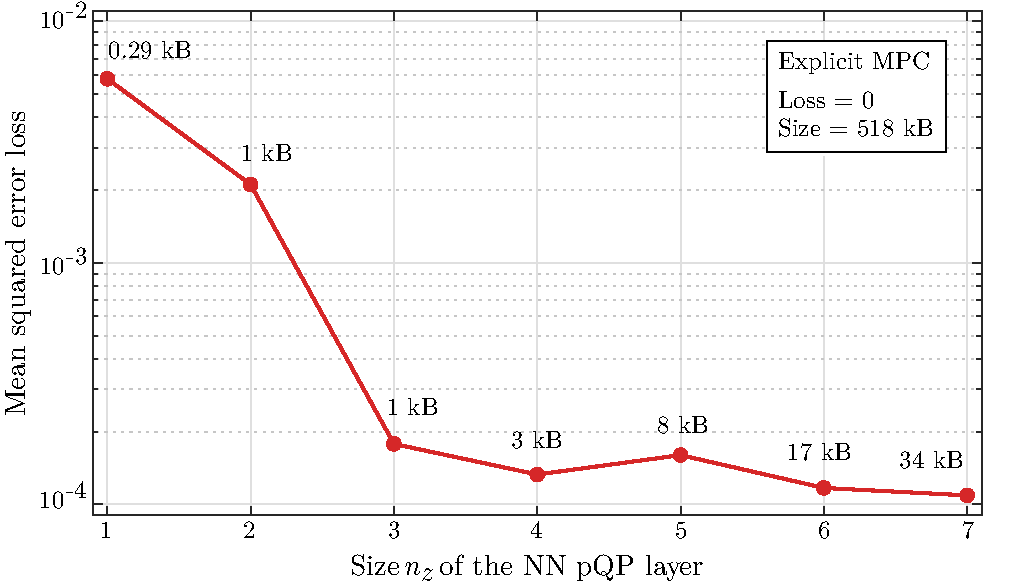
\includegraphics[scale=0.55]{../images/chap4_sim_res_loss_weight.pdf}    % The printed column width is 8.4 cm.
		\caption{Neural network training loss as a function of the	pQP layer size, and storage requirements associated with their PWA representations.} 
		\label{fig:pQP_mse_size}
	\end{center}
\end{figure}

\begin{figure}[!b]
	\vspace{0pt}
	\begin{center}
		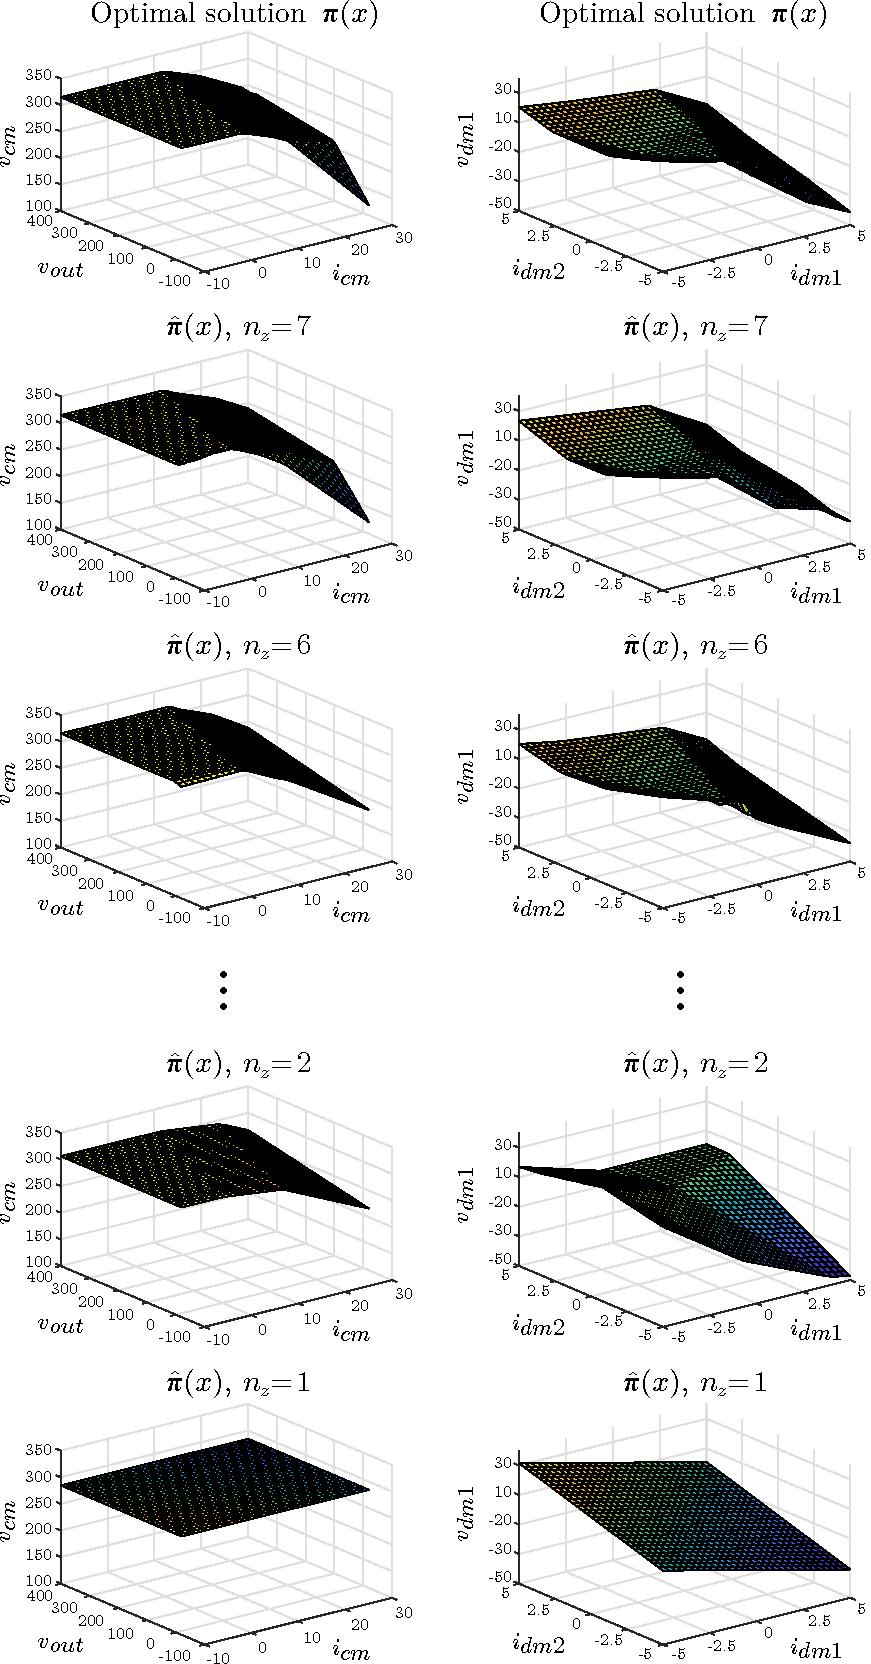
\includegraphics[scale=0.65]{../images/chap4_simres_surfs.pdf}    % The printed column width is 8.4 cm.
		\caption{Slices of the explicit MPC controller $\pi(x)$ and the pQP NN approximations $\hat\pi(x)$ for two control variables: $v_{cm}$ (left) and $v_{dm1}$ (right).} 
		\label{fig:niceSlices}
	\end{center}
\end{figure}

Analyzing Figure~\ref{fig:pQP_mse_size}, one sees that an increase in the $n_z$ size tends to lead to a better fit. This however does not always translate to a decrease in the final loss since the training process is affected by the weights initialization, the randomized nature of the optimizer, among other factors. As for the size complexity of the pQP NN, the larger the $n_z$, the more space is needed to store it. Yet, only 6.5\% of the original explicit MPC space when $n_z=7$. Slices of the learned control policies are show in Figure~\ref{fig:niceSlices}, where it is possible to visually verify the increasing complexity of $\hat\pi(x)$ and how well it resembles the original $\pi(x)$ when $n_z = 7$.

In order to validate the pQP NN, the converter was simulated from four initial conditions and under all 7 different approximate controllers, and only the two largest ones ($n_z=$~6 and $n_z=$~7) met the target specifications given in the previous section. We refer to these two solutions as the \textit{viable learned controllers}. A phase portrait of the closed-loop system evolution over multiple steps starting from these initial conditions is depicted in Figure~\ref{fig:phasePortrait}. A summary of the two viable learned controller key figures is presented in Table~\ref{tab:pqp_params}, including their number of polytopic regions, storage requirements, worst-case computation time and the output steady-state (SS) error. Even though four initial states were given, the systems always converged to the same points and, hence, only one SS error is reported. Plus, the storage numbers also take into account all the remaining layers parameters. Analyzing the obtained results we see that the approximations drastically reduced the storage requirements by 93.4\% and 96.7\%, and sped up the average evaluation time by 83.7\% and 88.4\%, respectively for the $n_z=$~7 and $n_z=$~6 cases. The closed-loop trajectories with the proposed $\hat\pi(x)$ remained reasonably close to the scenario with the optimal $\pi(x)$, converging to nearby equilibrium points. In practice, steady-state errors are typically counteracted by using disturbance observers, which would require however learning an MPC controller defined on an extended parameter space \citep{pannocchia2015offset}.

\FloatBarrier

\begin{figure}[!h]
	\begin{center}
		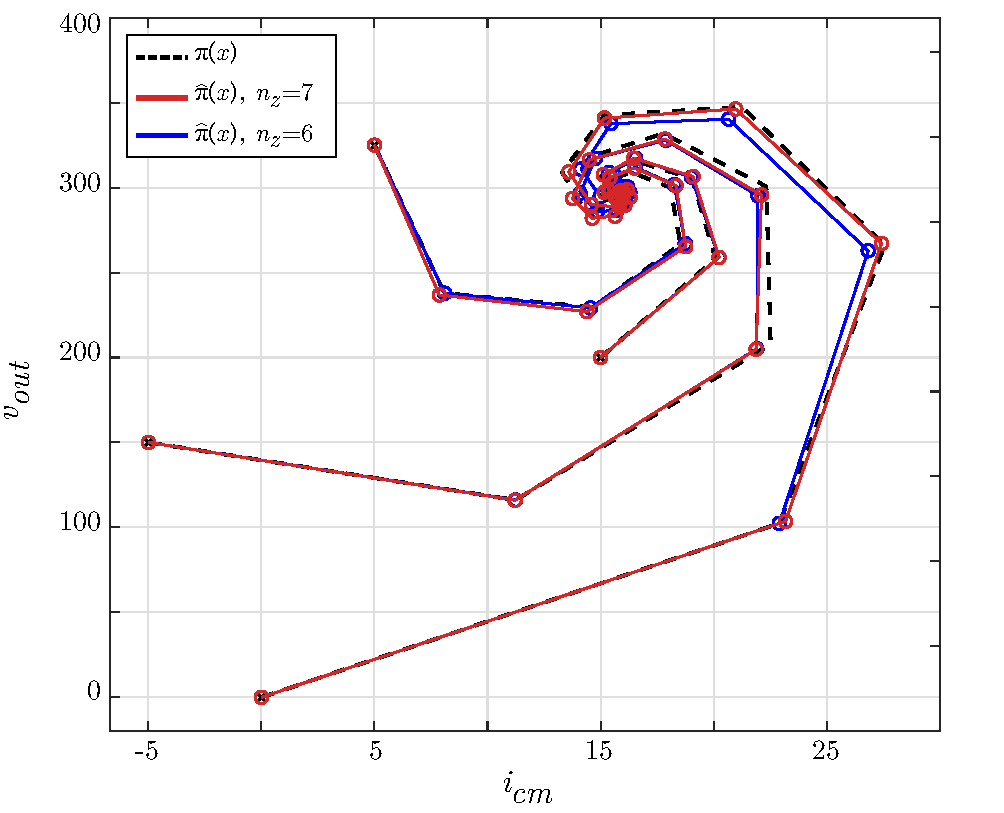
\includegraphics[scale=0.55]{../images/chap4_simres_phase_portrait.pdf} 
		\caption{Output voltage and common mode current phase portraits under the explicit MPC controller and the two viable pQP NN approximations.} 
		\label{fig:phasePortrait}
	\end{center}
\end{figure}

\begin{table}[h!]
	\begin{center}
		\caption{Explicit MPC and viable pQP NN controllers key features.} 
		\label{tab:pqp_params}
		\begin{tabular}{lcccc}
			\cmidrule[.15em](l{\tabcolsep}r{\tabcolsep}){1-5}
			Controller & Regions & Storage & Computational time & SS error \\
			\cmidrule[.05em](l{\tabcolsep}r{\tabcolsep}){1-5}
			$\pi(x)$ & 2'337 & 518$\,$kB & 12.9$\,$ms & 0\% \\ 
			\cmidrule[.05em](l{\tabcolsep}r{\tabcolsep}){1-5}
			$\hat\pi(x)$, $n_z$ = 7 & 107 & 34$\,$kB & 2.1$\,$ms & 0.59\% \\ 
			\cmidrule[.05em](l{\tabcolsep}r{\tabcolsep}){1-5}
			$\hat\pi(x)$, $n_z$ = 6 & 56 & 17$\,$kB & 1.5$\,$ms & 1.25\% \\ 
			\cmidrule[.15em](l{\tabcolsep}r{\tabcolsep}){1-5}
		\end{tabular}
	\end{center}
\end{table}

\FloatBarrier

\section{Experimental validation}

We now describe an experimental validation of the proposed pQP NN architecture, again in the context of power electronics. The system under study is a Buck converter, a building block of many switched-mode power supplies. The approximate MPC scheme was trained and then deployed on an inexpensive microcontroller, and the approach lead to an important start-up transient response enhancement.

\subsection{The system and the target predictive controller}
\label{sec.buck_conv}

A schematic representation of the Buck converter is shown in Figure~\ref{fig:buck} and its parameters are found in Table~\ref{tab.params_buck}. $V_{IN}$, $V_D$, $L$, and $C$ refer respectively to the input voltage, the diode forward drop, the inductance and the capacitance; whereas $R_{ON}$, $R_L$, $R_C$ and $R_{O}$ refer to the switch on-resistance, the inductor parasitic resistance, the capacitor parasitic resistance, and the output load. The purpose of this topology is to supply energy to the load at a voltage level equal or lower than the input source, which is accomplished by modulating the main switch.

We choose as state variables the inductor current and the output voltage
\begin{equation}
	x = \begin{bmatrix} x_1 & x_2 \end{bmatrix}^\top
	= \begin{bmatrix} i_L & v_O \end{bmatrix}^\top
\end{equation}
The power switch is operated at a constant frequency $f_{\text{sw}}$ and variable duty cycle, which is taken to be the control variable $u = \delta$. Following the classical time-averaging technique \citep{middlebrook1976general}, Kircchoff's circuit laws are first used to derive differential equations for both when the switch is closed, and when it is open. These are then averaged with $\delta$ and $(1-\delta)$ as weights, yielding
\begin{subequations}
	\begin{flalign}
		\dot{x}_1 = & \small{-\frac{R_L}{L}x_1 - \frac{1}{L}x_2 + \frac{V_{IN}+V_D}{L}u - \frac{R_{ON}}{L} x_1 u - \frac{V_D}{L} \label{eq.x1}} && \\[5pt]
		\dot{x}_2 = & \small{-\frac{R_C R_O R_L C + R_O L}{(R_C + R_O) L C}x_1 -\frac{R_C R_O C + L}{(R_C + R_O)L C}} x_2 + \frac{R_C R_O (V_{IN} + V_D)}{(R_C+R_O)L} u  &&\nonumber \\
		&- \frac{R_C R_O R_{ON}}{(R_C + R_O)L} x_1 u - \frac{R_C R_O V_D}{(R_C + R_O)L} \label{eq.x2} && 
	\end{flalign}
\end{subequations}

\begin{figure}[t!]
	\centering
	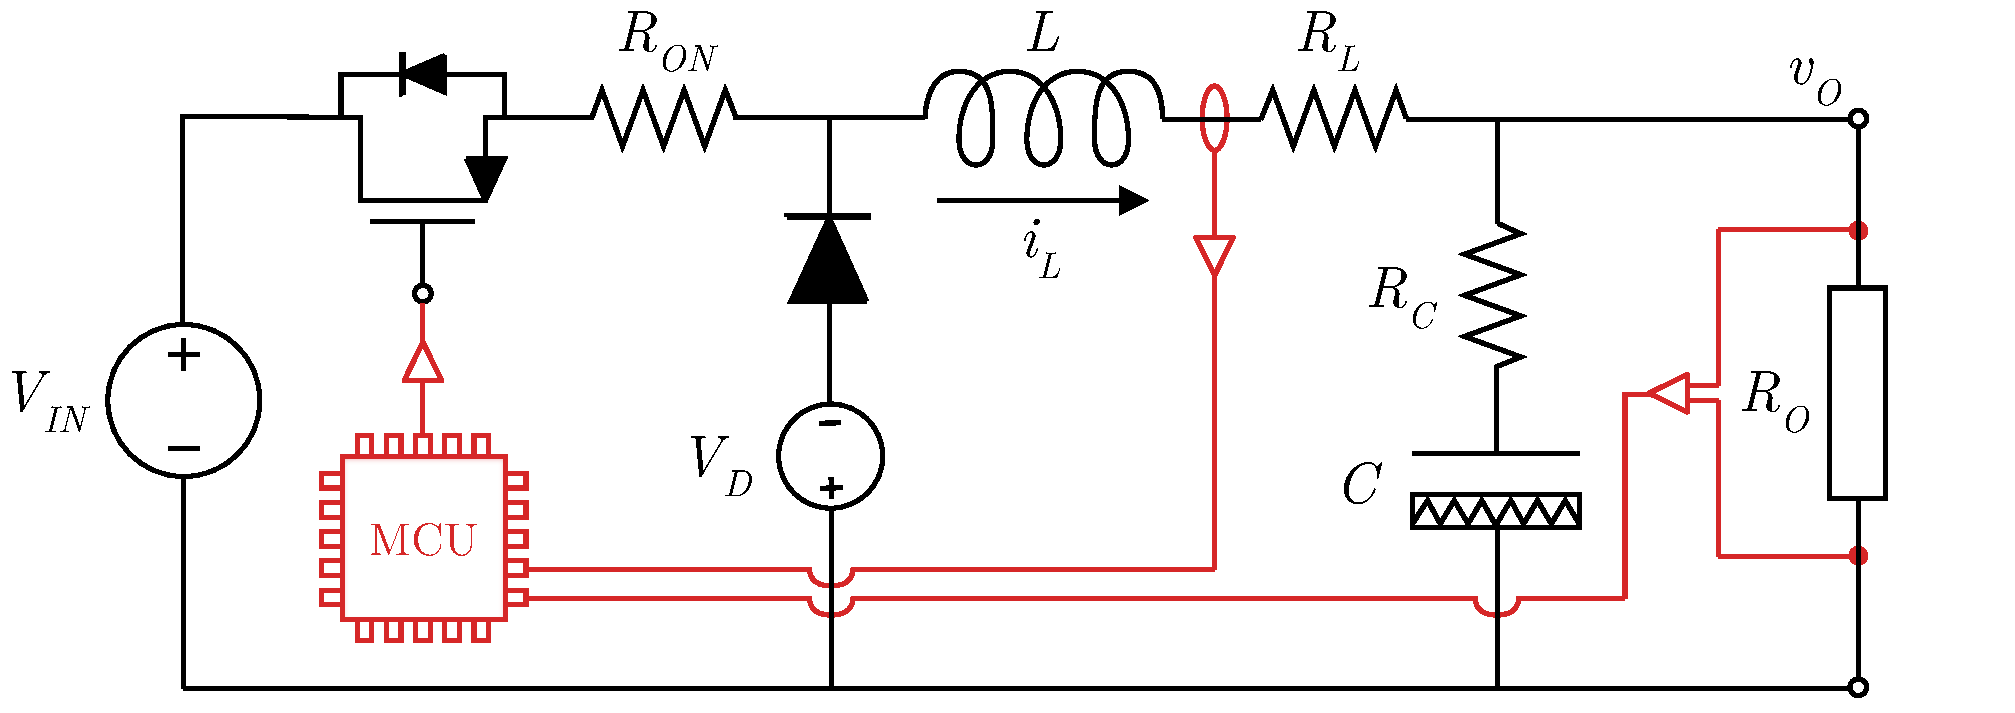
\includegraphics[width=0.8\linewidth]{../images/chap4_buck_schematic.pdf}
	\caption{A circuit diagram of the Buck converter including its parasitic resistances and the diode forward voltage drop. The feedback loop is closed by the microcontroller that implements our proposed pQP NN scheme.}
	\label{fig:buck}
\end{figure}

\begin{table}[t!]
	\begin{center}
		\caption{Parameters of the DC-DC converter} 
		\label{tab.params_buck}
		\begin{tabular}{cccccccccc}
			\specialrule{.15em}{.1em}{.1em} 
			$V_{IN}$ & $V_{OUT}$ & $V_{D}$ & $L$ & $C$ & $R_{ON}$ & $R_{L}$ & $R_{C}$ & $R_{O}$ & $f_{\text{sw}}$ \\
			\specialrule{.05em}{.1em}{.1em}
			15$\,$V & 5$\,$V & 0.1$\,$V & 10$\,$mH & 56$\, \mu$F &
			5$\,$m$\Omega$ & 2$\,\Omega$ & 330$\,$m$\Omega$ & 100$\,\Omega$ & 20$\,$kHz \\ 
			\specialrule{.15em}{.1em}{.1em}
		\end{tabular}
	\end{center}
\end{table}

The bi-linear expressions above are finally linearized around an equilibrium point, which is chosen by fixing the output voltage to the desired value $x_{2eq}$ and solving for the current and duty cycle steady-state values
%
\begin{align}
	x_{1eq} &= \frac{x_{2eq}}{R_O} \label{eq.x1eq}\\[5pt]
	u_{eq} &= \frac{R_O V_D + (R_L + R_O) x_{2eq}}{R_O(V_{IN}+V_D)-R_{ON} x_{2eq}} \label{eq.ueq}
\end{align}
%
Finally, \eqref{eq.x1} and \eqref{eq.x2} are expanded around $(x_{1eq},u_{eq})$ and only the linear terms are kept, leaving us with $\dot{x} = A_{ct} x + B_{ct} u$ where
\begin{align}
	A_{ct} & = \begin{bmatrix} 
		-\frac{R_L+R_{ON} u_{eq}}{L} & -\frac{1}{L} \\[5pt]
		-\frac{R_C R_O (R_L C - R_{ON} C u_{eq}) + R_O L}{(R_C + R_O) L C} & -\frac{R_C R_O C + L}{(R_C+R_O) L C}
	\end{bmatrix} 
	\\[5pt]
	B_{ct} & = \begin{bmatrix} 
		\frac{V_{IN} + V_D - R_{ON} x_{1eq}}{L} \\[5pt]
		\frac{R_C R_O(V_{IN}+V_D-R_{ON}x_{1eq})}{(R_C+R_O)L}
	\end{bmatrix}
\end{align}
As a last step, a discrete-time model $x_{t+1} = A x_{t} + B u_{t}$ is obtained by integrating the continuous-time dynamics using the zero-order hold method at $f_{\text{samp}} = 10\,$kHz.

The controller goal was to attain a fast start-up response\footnote{The start-up is defined as the system evolution from having zero energy in its storage elements to reaching the desired target output voltage.} with as little overshoot as possible and to regulate the output voltage $v_O$ to $v_{\text{eq}}=5\,$V. Furthermore, an inductor maximum current constraint of 200$\,$mA and maximum voltage constraint of $7\,$V were imposed. The prediction horizon was $N = 10$ and the standard quadratic cost \eqref{eq.MPC_cost_tracking} was employed with weights $Q = \text{diag}(90,1)$, $R = 1$, and $P$ as the solution of the associated discrete-time algebraic Ricatti equation. The reference equilibrium values $x_{\text{eq}} = \begin{bmatrix} 0.05 & 5 \end{bmatrix}^\top$, $u_{\text{eq}} = 0.3379$ were used, along with the constraints
\begin{align}
	x^{\text{min}} &= 
	\begin{bmatrix} i_L^{\text{min}} & v_O^{\text{min}}\end{bmatrix}^\top = 
	\begin{bmatrix} 0 \, \text{mA} & 0 \, \text{V}\end{bmatrix}^\top \\[3pt]
	x^{\text{max}} &= 
	\begin{bmatrix} i_L^{\text{max}} & v_O^{\text{max}}\end{bmatrix}^\top = 
	\begin{bmatrix} 200 \, \text{mA} & 7 \, \text{V}\end{bmatrix}^\top \\[3pt]
	u^{\text{min}} &= 0, \quad u^{\text{max}} = 1 
\end{align}
%
and $x_N \in \mathbb{X}_N$, with $\mathbb{X}_N$ being the maximum invariant set for the dynamical system under the corresponding LQR control law.

After computing the explicit solution $\pi(x)$ with the MPT toolbox, the map was found to have $70$ regions as shown in Figure~\ref{fig.approx_results}. Although this number may not seem too large for a general purpose computer, it can still be challenging for certain microcontrollers (MCU) to handle, especially since the algorithm has to be executed in under 100$\,\mu$s. In fact, pQP NN approximations can be beneficial to the power supply industry since the computing platforms are often MCUs with limited memory and relatively slow clocks.

%The matrix weights were $\mathcal{X}_N$ was chosen to be the the system's maximal invariant set under the corresponding LQR policy. Both the terminal ingredients ($P$ and $\mathcal{X}_N$) can be easily calculated with the aid of the Multi-Parametric Toolbox (MPT) \cite{mpt} for MATLAB, and are employed to ensure recursive feasibility and closed-loop stability \cite{rawlings2017model}.
%
%As a final step, the MPC controller \eqref{eq:mpcFormulation} was solved off-line using MPT, which yielded a piecewise-affine (PWA) function $\pi(x)$ that maps states directly to optimal control inputs. As well known in the area of explicit model predictive control \cite{alessio2009survey}, this function partitions the space of feasible states $\mathcal{X}$ into regions described by sets of linear inequalities. Then, applying the predictive controller on-line boils down to implementing the look-up table of feedback gains
%\begin{align}
%	u = \pi(x) = 
%	\begin{cases}
%		F_1 x + g_1, &\text{if } x \in \text{region } 1 \\
%		\quad \; \dots & \qquad \dots \\
%		F_M x + g_M, &\text{if } x \in \text{region } M \\
%	\end{cases}
%	\label{eq.PWA}
%\end{align}
%
%As provided by MPT, the computed control policy $\pi(x)$ had $M = 70$ regions, a number too large to be embedded into the target MCU due to the large storage and computational demands (more details are given in Section~\ref{sec.complRed}). These implementation issues motivate the use of our PWA-NN complexity reduction scheme.

\subsection{Learning the optimal controller and deploying the algorithm}

The explicit control law $\pi(x)$ was sampled in order to collect a set of state-control pairs for a total of $5'000$ points. A uniform distribution over the set of feasible states was used throughout. In order to achieve a balanced learning over the domain, the currents and voltages values that formed the initial states were normalized to a range of $[0,1]$ The same software framework, loss function and optimization algorithm from the last example were used with a mini-batch size of $50$ and $150$ epochs. All pQP weights were initialized randomly. The code was run on a 3.1~GHz Intel Core i7 laptop with 16~GB 2133~MHz of memory, and training the network once took on average $35\,$mins without any GPU acceleration. The size $n_z$ was gradually increased to improve the fitting results and with $n_z = 3$, after only $5$ re-initializations, a low mean squared error training loss was attained: $1.66\times 10^{-7}.

Both the map and the domain partition of the pQP NN can be seen in Figure~\ref{fig.approx_results}, where the number of regions was reduced from 70 to 6, and the memory required to store the control law, 9.25~kB to 528~B. This last improvement can be particularly useful to fit all the parameters in specialized, small memory slots that are closed to the processor core than the main memory. Visually inspecting the surfaces shown in Figure~\ref{fig.approx_results}, one can note how similar the two are. As pointed out in Section~\ref{sec.properties_approx}, the domain of the learned controller is larger than the original one, which can be verified in the partition plots. We underline that the 6 regions of the pQP NN are associated with the pQP layer L2 and that the map $\hat\pi(x)$ is composed of other elements such as the linear layers and the saturation element in L4. Finally, closed-loop simulations based on the nominal system model were performed from different initial conditions around the origin to test the learned controller, after which we proceeded to the embedded implementation phase.

%Again, the \texttt{PyTorch} and \texttt{OptNet} packages for Python were employed to code the NN and mini-batch stochastic gradient descent was used to train it. The batch size was chosen to be $50$, and the whole dataset was presented to the algorithm a total of $150$ times, i.e., $150$ epochs. In order to achieve a balanced learning throughout the domain, the currents and voltages values that formed the input locations $x_d$ were normalized to a range of $[0,1]$. Furthermore, all trainable weights were initialized randomly. The code was run on a 3.1~GHz Intel Core i7 laptop with 16~GB 2133~MHz of memory. As previously explained, we gradually increased the size $n_z$ of the PWA-NN. Training the network once took approximately $35\,$mins without any GPU acceleration. With $n_z=3$, after only $5$ initializations, the network presented a very low mean squared error training loss: $1.66\times 10^{-7}$. As for the testing phase, we calculated the true outputs $u = \pi(x)$ and the predicted values $\hat{u} = \hat{\pi}(x)$ on a grid of points; the latter were capable of closely reproducing the original controller as shown in the top plots of Figure~\ref{fig:part}.
%
%In order to assess the complexity of the learned controller, its L2 layer was converted into a PWA function using the MPT toolbox. As can be seen from lower plots in Figure~\ref{fig:part}, the number of region was greatly reduced: from 70 in the original partition to 6 in the simplified one, a reduction of 91\%. The total memory required to store the control law parameters was reduced from 9.25~kB to 528~B. The latter quantities were calculated by counting the total number of constants needed to describe all the inequalities that compose the polytopes and the remaining NN layers, and assuming that each of them occupies 1 \textit{word} of space.

A photo of the Buck converter prototype designed and assembled in the Automatic Control Laboratory at EPFL is presented in Figure~\ref{fig.prototype}, and its parameters are listed in Table~\ref{tab.params_buck}. The current monitoring circuit consisted of a $150\,$m$\Omega$ shunt resistor and a INA282 differential amplifier, whereas the output voltage was simply scaled down by means of a voltage divider with no isolation. In order to control the step-down converter, an STM32L476 was chosen as the embedded platform: the MCU runs at 80 MHz, it has a 32-bit RISC architecture and two independent 12-bit ADC channels. The firmware was written in an interrupt-driven, bare metal fashion and was triggered at 10 kHz. To avoid using raw measurements and also to filter noise, the ADCs were operated at a faster pace and 5 consecutive readings were averaged before being sent to the pQP NN routine. Only integers were used to encode all control law parameters (the polytopes and feedback gains) and the direct memory access peripheral was activated to link the ADC blocks directly to memory. As the PWA description of the pQP layer only featured 6 regions, a simple sequential search was employed. All these steps were needed to ensure that all instructions could be executed within the 100$\,\mu$s time slot.

The natural open-loop start-up transient is reported in Figure~\ref{fig.buck_exp_res} (top), which shows peaks of 7.97$\,$V and 330$\,$mA, corresponding respectively to overshoots of 59\% and 660\%. In Figure~\ref{fig.buck_exp_res} (middle), how the transient response was improved under the pQP NN control law, with voltage and current peaks of 5.16$\,$V and 202$\,$mA, respectively. By examining the yellow curves, one sees that its initial derivative was reduces from the top to the middle oscilloscope prints, indicating a slower flow of energy from the source to the output capacitor. This was expected as the inductor current had to satisfy the constraints and was capped\footnote{The average dynamical model developed for the converter in Section~\ref{sec.buck_conv} predicts the average state values between the ON and the OFF semi-cycles, whereas the 202$\,$mA peak current reported by the oscilloscope are absolute.}. Yet, the output voltage settling time was reduced from 6.73$\,$ms to 2.33$\,$ms. Lastly, we have also examined the execution time of the controller routine, responsible for averaging ADC samples, locating the pertinent PWA region, computing the control action and updating the PWM peripheral with the new duty cycle value. The execution period did not show much variance and lasted between 22.0$\,\mu$s and 27.5$\,\mu$s as shown by the blue signal in Figure~\ref{fig.buck_exp_res} (bottom). In a practical scenario, this is rather positive since the MCU core would not be always
busy, but would have time available to execute additional side tasks.

\begin{figure}[!t]
	\centering
	\vspace{20pt}
	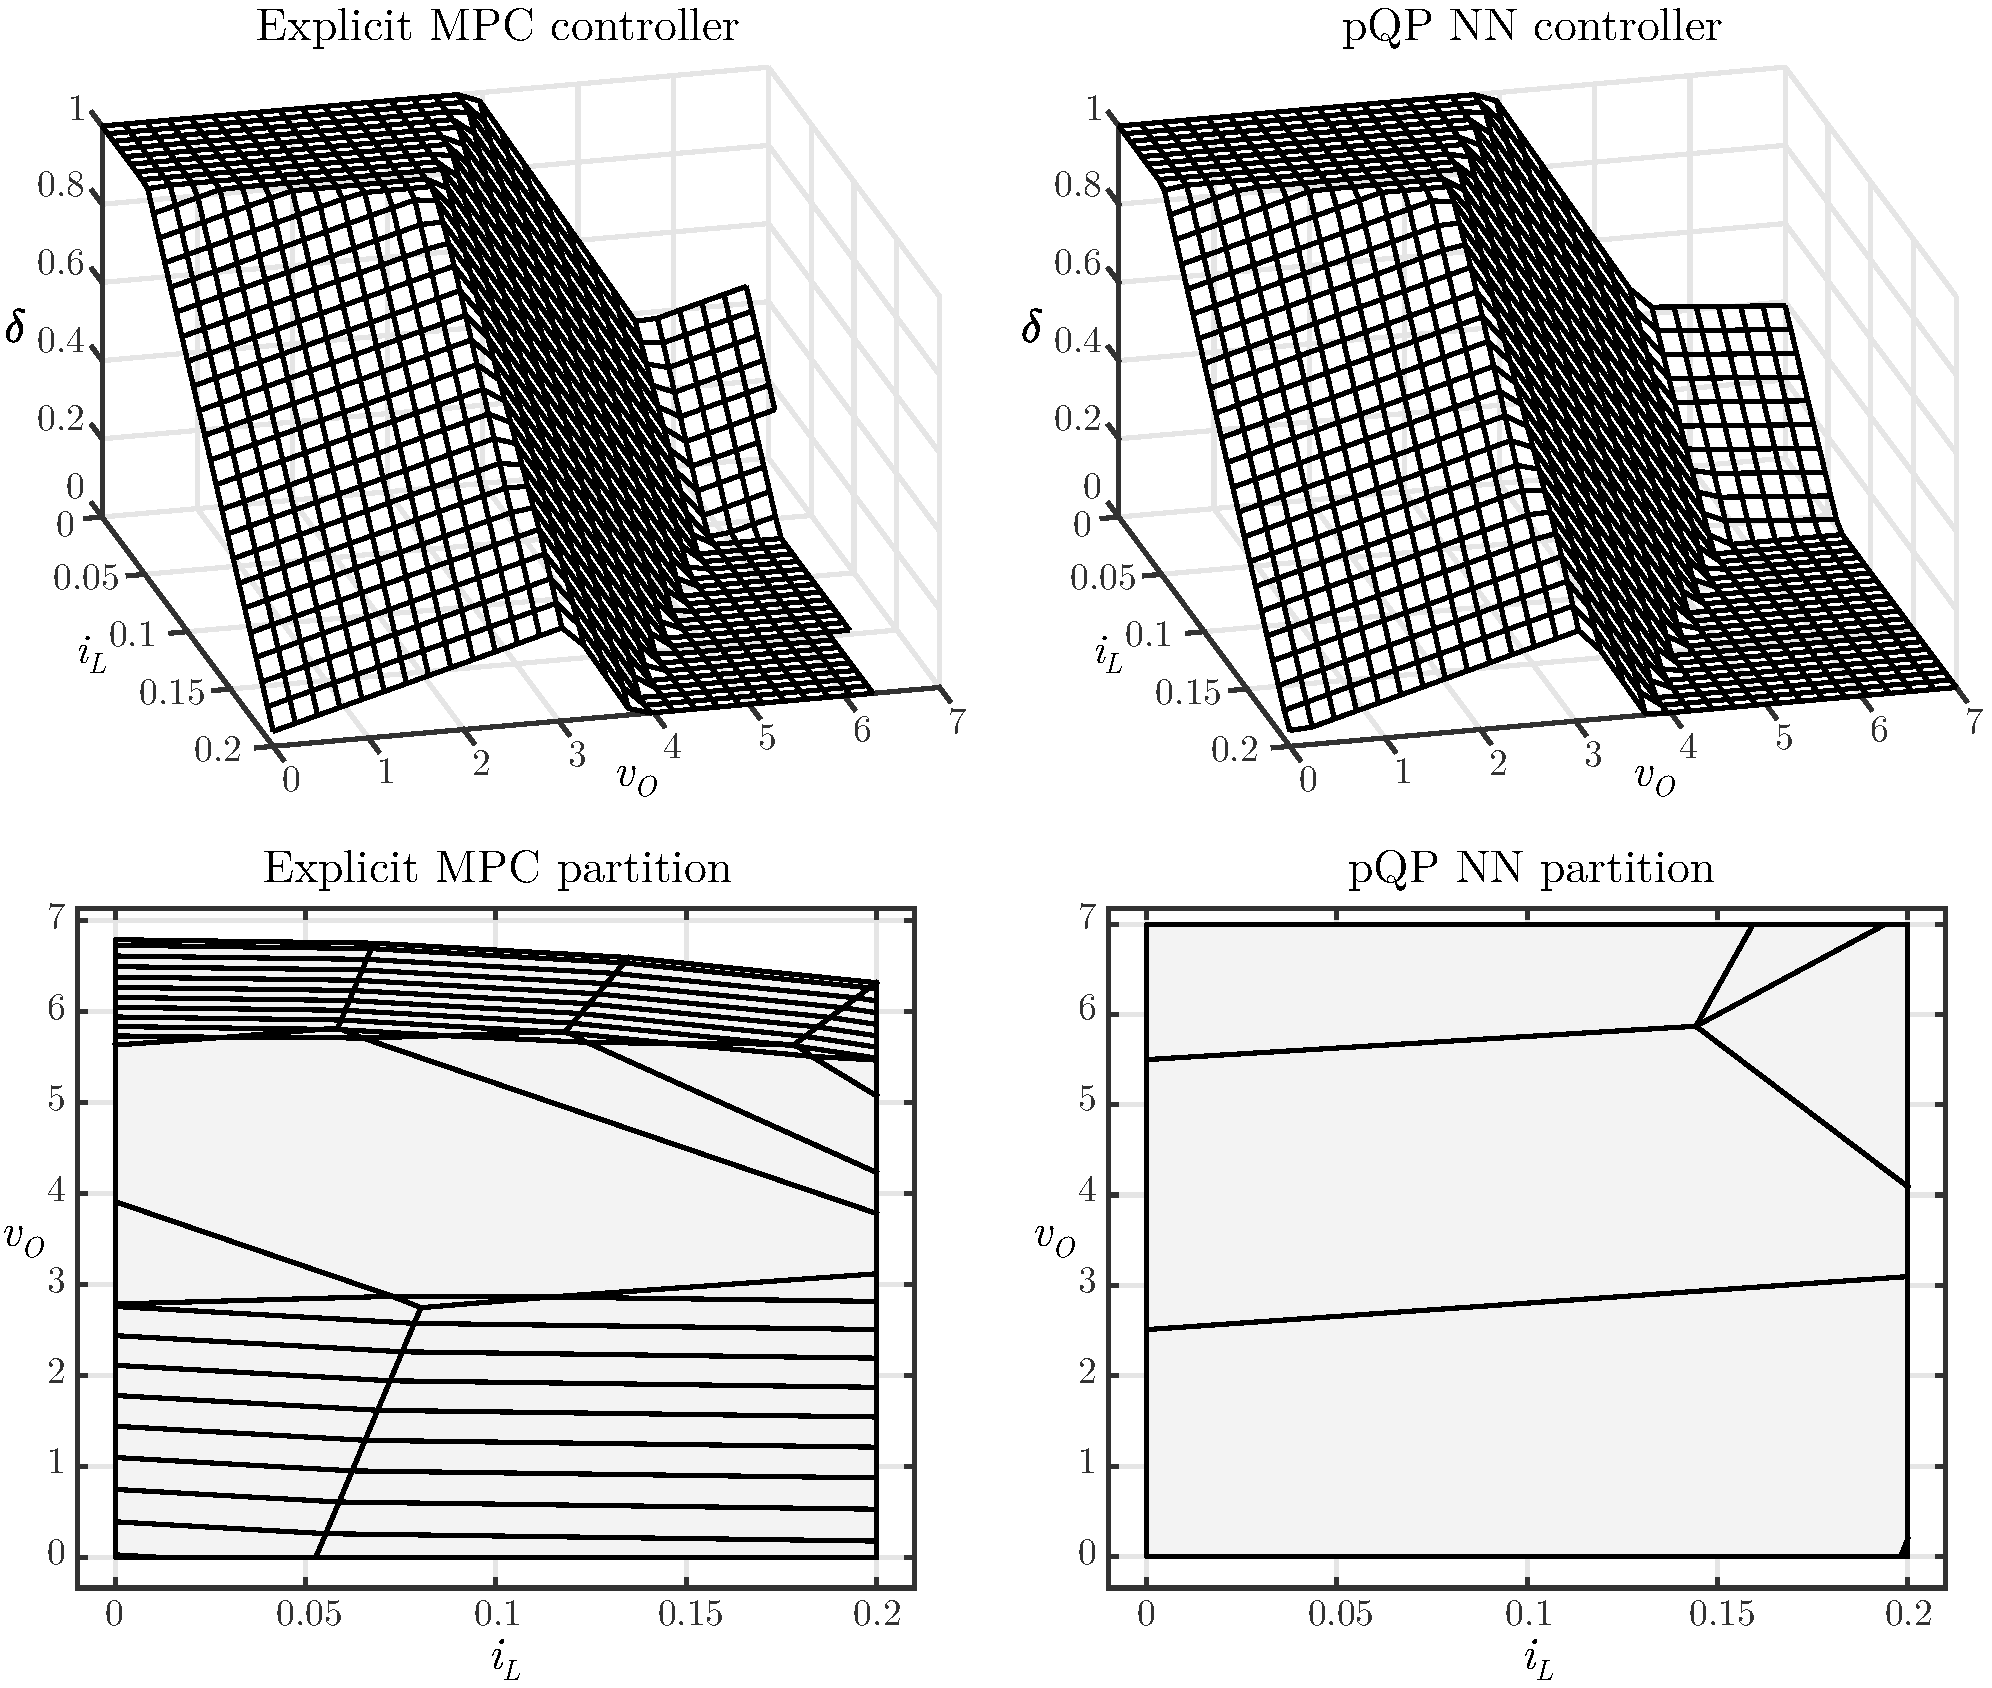
\includegraphics[scale=0.37]{../images/chap4_approx_results.pdf}
	\caption{The original explicit MPC map and its domain partition (left), and the learned pQP NN map and its domain partition (right).}
	\label{fig.approx_results}
	\vspace{22pt}
	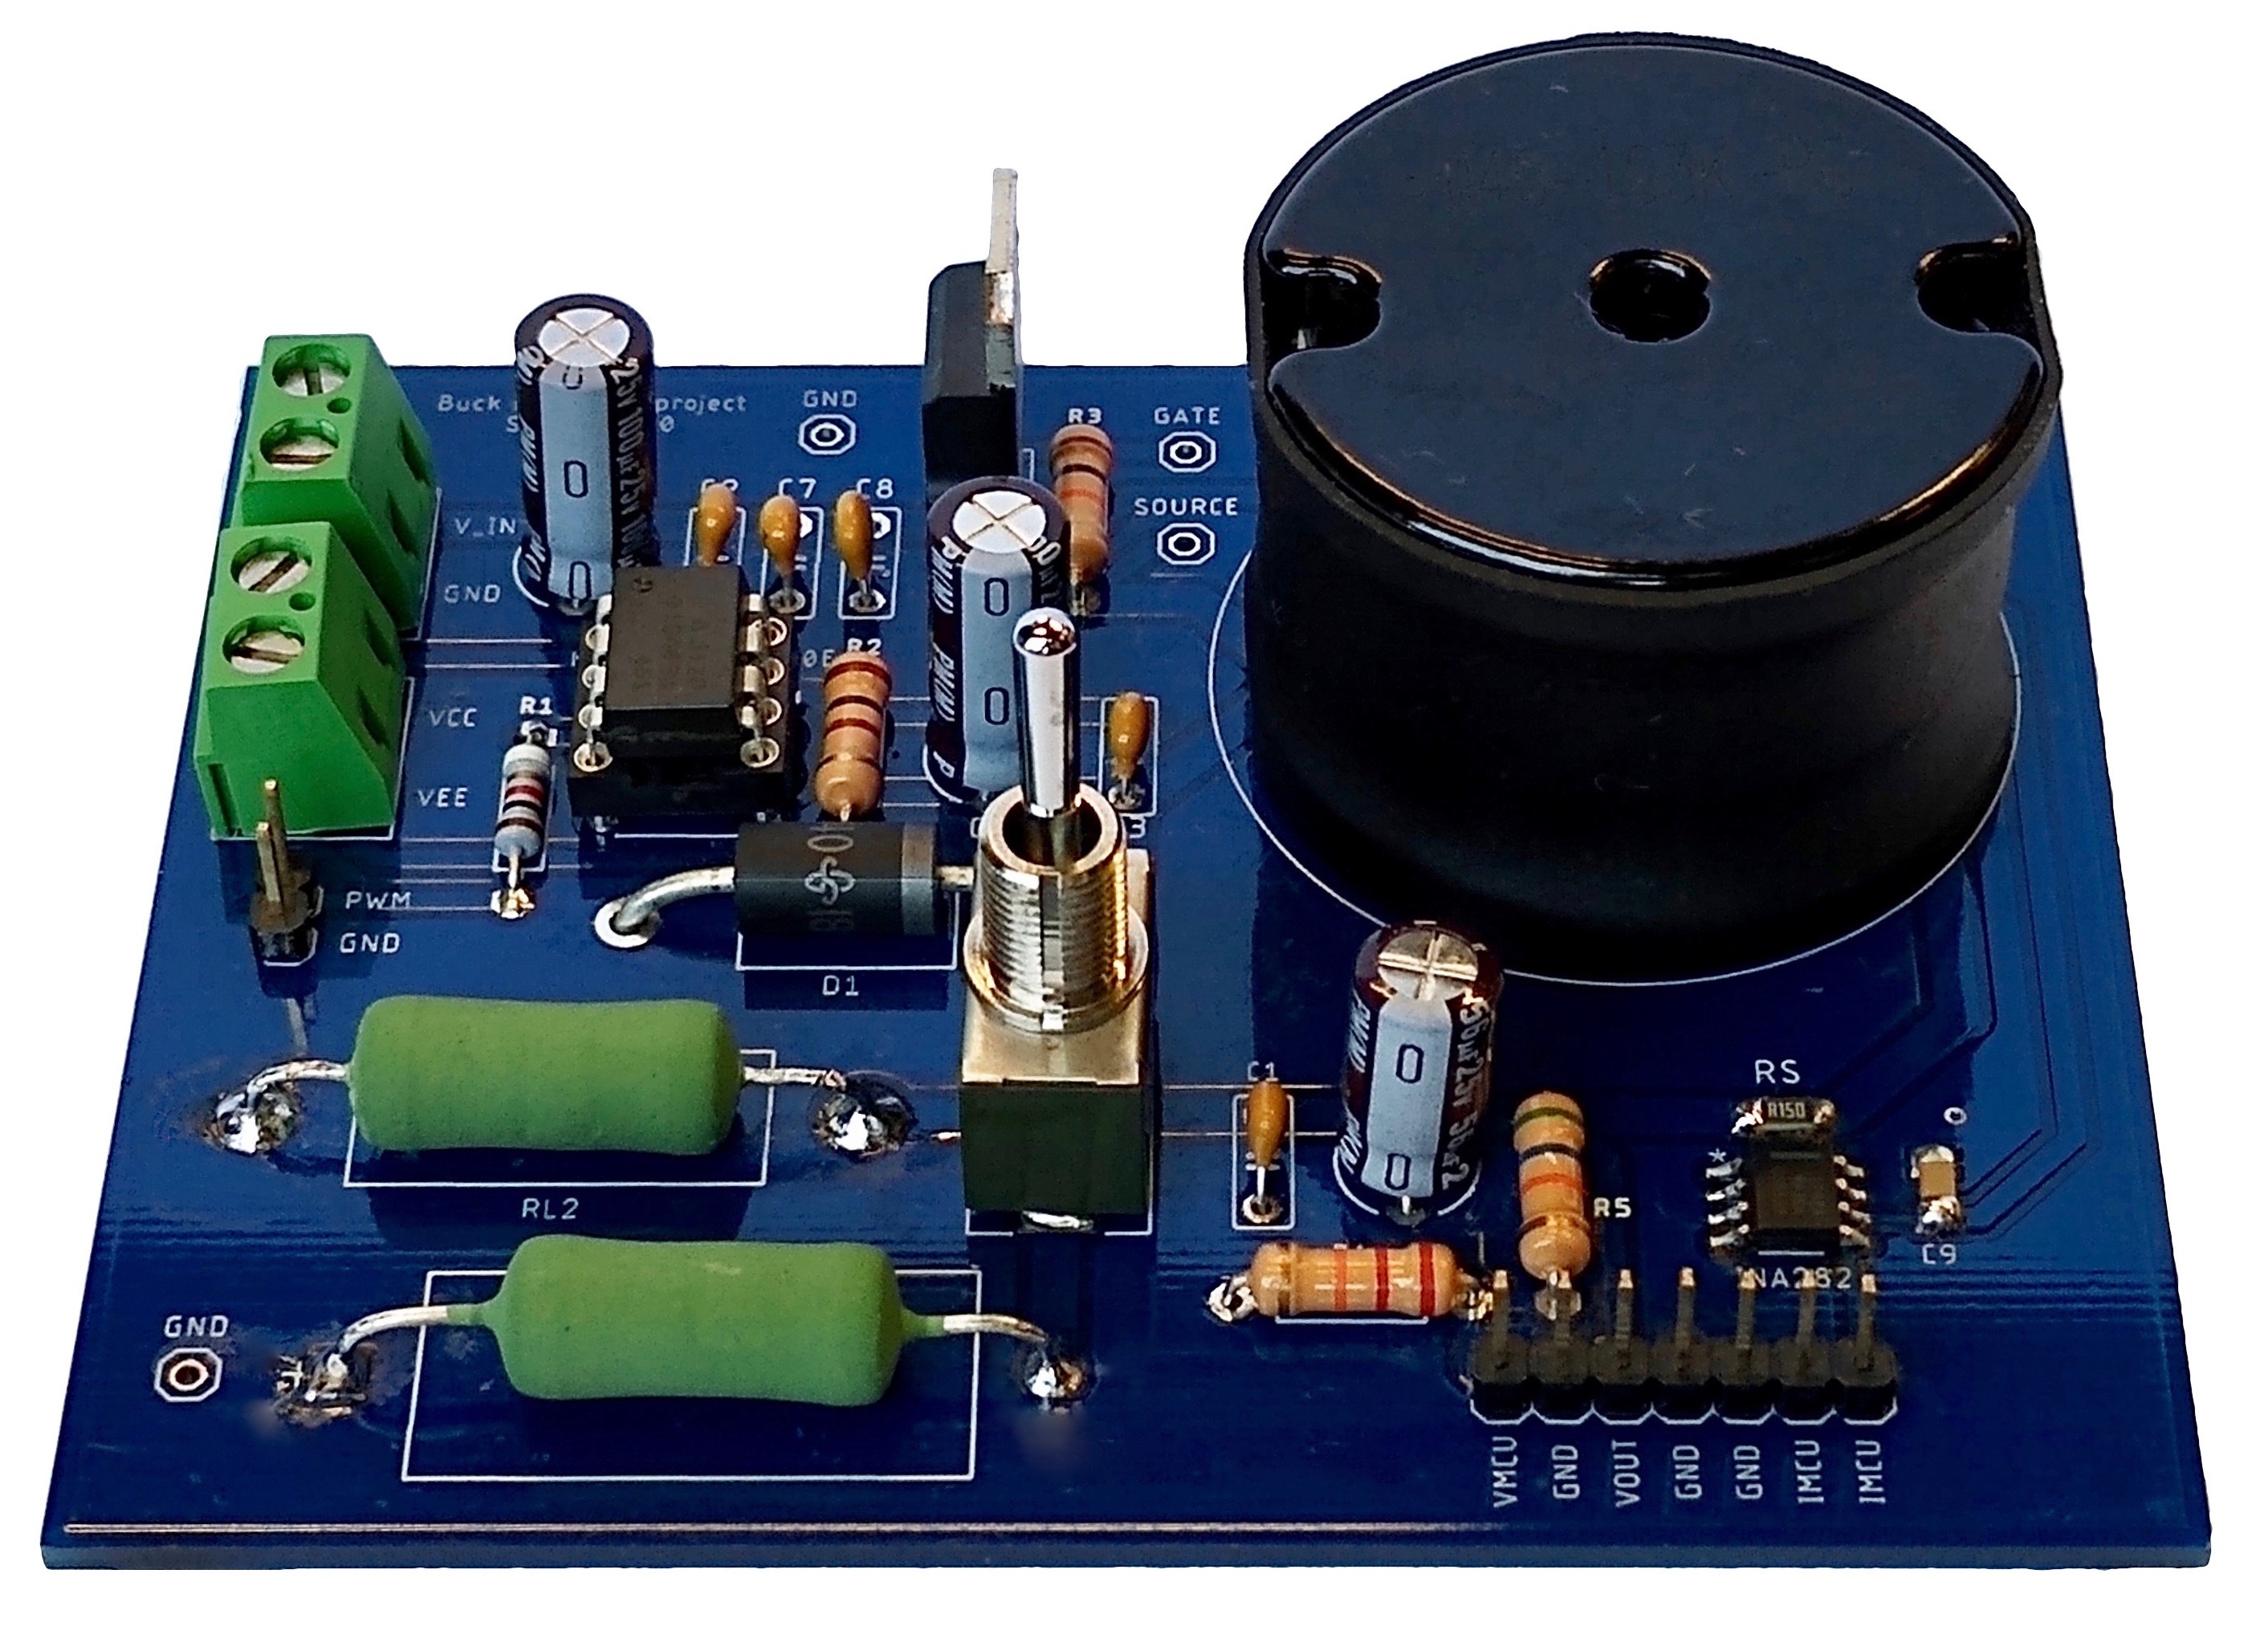
\includegraphics[width=0.66\linewidth]{../images/chap4_buck}
	\caption{A picture of the Buck converter prototype designed and assembled in the Automatic Control Laboratory at EPFL.}
	\label{fig.prototype}
\end{figure}

\begin{figure}[p] 
	\vspace{35pt}
	\centering
	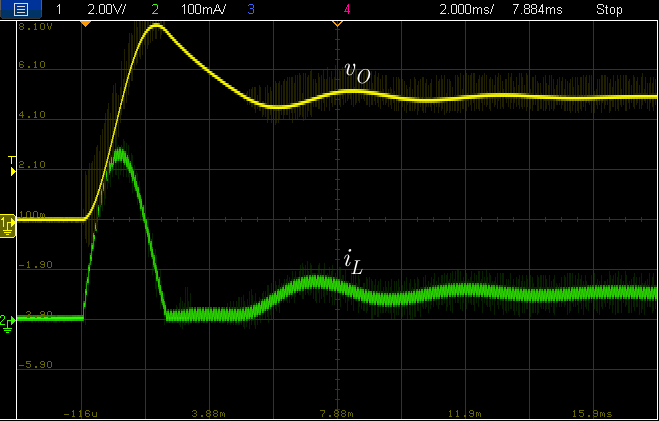
\includegraphics[width=0.65\linewidth]{../images/chap4_scope_ol} \\[10pt]
	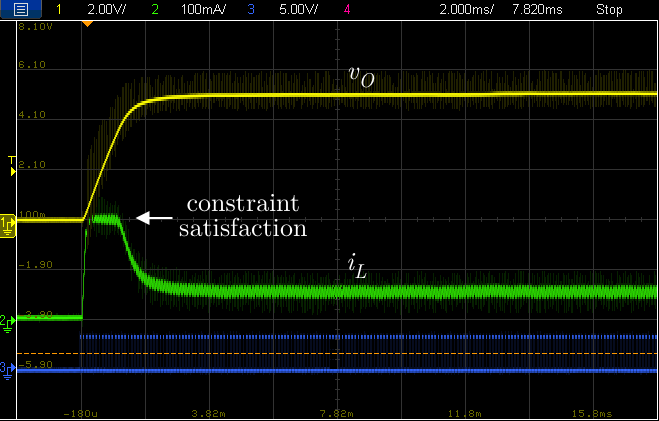
\includegraphics[width=0.65\linewidth]{../images/chap4_scope_cl1} \\[10pt]
	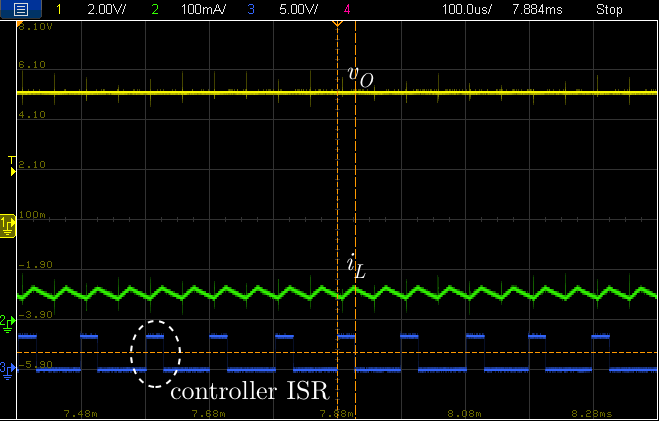
\includegraphics[width=0.65\linewidth]{../images/chap4_scope_cl2} \\[10pt]
	\caption{Open-loop start-up response (top), closed-loop start-up response (middle), and a close-up view of the closed-loop start-up response highlighting individual switching cycles and the controller interrupt service routine (ISR) execution time of approximately 27$\;\mu$s.}
	\label{fig.buck_exp_res}
\end{figure}

\section{Conclusions and outlook}

In this chapter, we put forward a novel neural network architecture featuring a pQP layer to approximate linear MPC controllers. Similarly to the process of computing an explicit MPC control law, a PWA description of the pQP problem can be obtained, and its complexity can be controlled by the user and regarded as a network hyperparameter. As a result, once the architecture is trained, a forward pass simplifies to evaluating a chain of affine and PWA expressions, without requiring solving any optimization problem. Additionally, we showed that the pQP layer is a suitable inductive bias for MPC, indeed, it was shown that any linear MPC policy can be learned exactly by the proposed network given a suitable size.

Two application examples in the domain of power electronics were presented, showcasing the merit of the MPC learning scheme. First, through simulations, the effects of the pQP layer size on the fitting error, memory requirements and number of regions was investigated; and the simplified control laws were tested by comparing closed-loop trajectories. Promising results were observed, suggesting that complex PWA functions with thousands of regions can be fit with around one hundred regions without a significant deterioration of the dynamical system response. Second, a smaller-scale problem was tackled, but this time involving a real power supply. The pQP NN was used to reduce by 90\% the complexity of the original explicit control law and was subsequently deployed on a low-cost microcontroller. The necessary computations were carried out in under $27\,\mu$s and the transient response was substantially enhanced.  Finally, our experiments included a trajectory where a current constraint was activated and not violated by the pQP NN approximate policy.

From a theoretical perspective, one aspect that could be researched in the future is the link between the training cost and the worst-case approximation error. Intuitively, the training loss carries information between the approximation discrepancy at the sample locations. In addition, it is known that both the ground-truth and the approximator are continuous maps over compact sets. Therefore, with an appropriate sampling strategy, out-of-samples error bounds could potentially be established for the pQP NN scheme based solely on the training error. Another direction that could be taken regard is to devise initialization strategies for the pQP layer. In effect, this would amount to finding suitable dual problems that approximate well the MPC dual while being smaller in size. The envisioned advantage is a faster convergence of the network to better solutions.

From a practical viewpoint, we see at least two possible paths to be explored. One concerns the advantages of adopting the pQP NN over a generic deep network (DNN) with ReLU activation functions. We suspect DNNs to require in general a large number of neurons and to result in a final map with a considerably larger number of regions and kinks, whereas we expect our scheme to be more economical. Second, we strongly believe that the problem of approximating mixed-integer MPC problems deserves more attention. In particular, users of the so-called finite-set MPC formulation \citep{karamanakos2019guidelines} that has become popular in recent years, have often to restrict their prediction horizons to one for computational reasons \citep{kim2015offset}. We suspect that modern classifiers could be employed to efficiently learn the optimal control actions from a discrete set in long horizon formulations, unlocking important performance gains.

%Two examples were presented to showcase the capabilities of the pQP NN to greatly simplify MPC controllers while delivering good performance. Our experimental investigation demonstrated that the technique can be deployed on inexpensive hardware platforms to reliably control dynamical systems with fast dynamics.
%The use of alternative machine learning models to learn mixed-integer MPC problems such as the ones arising in finite-control set MPC.

\pagebreak

\section{Appendix}

As mentioned in Section~\ref{sec.chap4_intro}, a fair number of linear MPC simplification techniques exists, most of which were proposed in the late 2000s and early 2010s. Our goal in this appendix is to compare the pQP NN learning strategy with the methods implemented in the MPT toolbox \citep{herceg2013multi} and that can be easily accessed through the \texttt{simplify()} function. The reader is referred to the MPT documentation for details on each method and the associated publications. Herein we will adopt an user's perspective and simply apply each of them.

First, consider the MPC formulation used in our experimental investigation (Section~\ref{sec.buck_conv}), which has a PWA form $\pi(x)$ composed of $70$ regions. Four different simplification techniques were applied to $\pi(x)$ and the resulting number of regions was counted. Additionally, a grid of 6'561 points was laid on the domain to collect new state-control pairs and compute an average mean squared validation error. The results are displayed in Table~\ref{tab.extra_simpl_res1} and are compared to the pQP NN with $n_z=3$ shown in Figure~\ref{fig.buck_exp_res}. The \texttt{clipping} method returned a controller with less than haft of the original complexity, but with comparatively high validation error. The \texttt{greedy} strategy lead to a map with only $20$ regions and virtually no validation error. The last three approaches could be considered as equally competitive since they delivered maps with a low number of regions and low validation error.

Next, the MPC formulation was modified with weight matrices $Q = \text{diag}(1, 1)$, $R = 100$ and a horizon of $N = $100. In this case, the explicit MPC controller $\pi(x)$ had $189$ regions. This second batch of results is displayed in Table~\ref{tab.extra_simpl_res2}. As can be seen, most of the MPT techniques failed to simplify $\pi(x)$ and essentially preserved the original number of regions, hence the low validation error. The \texttt{fitting} approach was the only one able to significantly reduce the map complexity while attaining a good fit. The pQP NN, on the other hand, lead to a PWA function with the same 5 partitions and less than half of the validation error when compared to the \texttt{fitting} scheme, although in the same order of magnitude.

From our numerical experiments, we have observed that some simplification schemes rely on features that are often observed in simplified case studies such as clear saturation regions, or neighboring parts sharing the same affine gains. On the other hand, the pQP NN is a more general approximator that does not explicitly make use of that information. As a result, the pQP NN tends to return good results in a large number of cases, whereas the specialized techniques sometimes work well, but fail in other situations. Nevertheless, it is fair to mention that training a single pQP network took around 30 minutes, whereas executing any of the \texttt{simplify()} methods, less than 30 seconds.

\FloatBarrier 

\begin{table}[t]
	\begin{center}
		\caption{Complexity reduction results for an explicit MPC control law $\pi(x)$ with 70 regions.} 
		\label{tab.extra_simpl_res1}
		\begin{tabular}{ccc}
			\specialrule{.15em}{.1em}{.1em} 
			MPT method & num. regions & validation error \\
			\specialrule{.15em}{.1em}{.1em}
%			\texttt{orm}  & - & $< 10^{-30}$ \\
%			\specialrule{.05em}{.1em}{.1em}
			\texttt{clipping} & 25 & $1.49\,10^{-4}$\\
			\specialrule{.05em}{.1em}{.1em}
			\texttt{greedy} & 20 & $< 10^{-20}$ \\
			\specialrule{.05em}{.1em}{.1em}
			\texttt{separation} & 7 & $< 10^{-20}$ \\
			\specialrule{.05em}{.1em}{.1em}
			\texttt{fitting} & 5 & $3.03\,10^{-8}$ \\       
			\specialrule{.05em}{.1em}{.1em}
			pQP NN & 6 & $6.07\,10^{-5}$ \\
			\specialrule{.15em}{.1em}{.1em}
		\end{tabular}
	\end{center}
\end{table}

\begin{table}[t!]
	\begin{center}
		\caption{Complexity reduction results for an explicit MPC control law $\pi(x)$ with 189 regions.} 
		\label{tab.extra_simpl_res2}
		\begin{tabular}{ccc}
			\specialrule{.15em}{.1em}{.1em} 
			MPT method & num. regions & validation error \\
%			\specialrule{.15em}{.1em}{.1em}
%			\texttt{orm}  & 182 & $< 10^{-20}$ \\
			\specialrule{.05em}{.1em}{.1em}
			\texttt{clipping} & 187 & $6.31\,10^{-8}$\\
			\specialrule{.05em}{.1em}{.1em}
			\texttt{greedy} & 183 & $< 10^{-20}$ \\
			\specialrule{.05em}{.1em}{.1em}
			\texttt{separation} & 187 & $< 10^{-20}$ \\
			\specialrule{.05em}{.1em}{.1em}
			\texttt{fitting} & 5 & $3.71\,10^{-4}$ \\       
			\specialrule{.05em}{.1em}{.1em}
			pQP NN & 5 & $1.75\,10^{-4}$ \\
			\specialrule{.15em}{.1em}{.1em}
		\end{tabular}
	\end{center}
\end{table}
%Here we present additional results that illustrate the potential
%of the proposed technique. Firstly, the MPC controller param-
%eters described in Section III were modified to Q = diag(1, 1),
%R = 100 and a horizon of N = 100. The predictive controller
%explicit form π (x) had M = 189 regions. Next, all simplifi-
%cation techniques available on MPT were applied to π (x)—
%these can be accessed through the simplify() command.
%The results are shown in Table 2, where the validation error
%indicates the mean squared error calculated on a grid of 6561
%points. As can be seen, most of the MPT techniques failed in
%simplifying π (x) and essentially preserved the original num-
%ber of regions. The ‘fitting’ approach however drastically re-
%duced the number of regions with a reasonably low validation
%error.
